\documentclass[journal]{IEEEtran} % use the `journal` option for ITherm conference style

\usepackage{cite}
\usepackage{amsmath,amssymb,amsfonts}
\usepackage{algorithmic}
\usepackage{graphicx}
\usepackage{textcomp}
\usepackage{xcolor}
\def\BibTeX{{\rm B\kern-.05em{\sc i\kern-.025em b}\kern-.08em
    T\kern-.1667em\lower.7ex\hbox{E}\kern-.125emX}}
\usepackage{color}
\usepackage{algorithm}
\usepackage{float}
\usepackage{listings}
\usepackage{dblfloatfix}
\def\BibTeX{{\rm B\kern-.05em{\sc i\kern-.025em b}\kern-.08em
    T\kern-.1667em\lower.7ex\hbox{E}\kern-.125emX}}

\definecolor{mygreen}{rgb}{0,0.6,0}
\definecolor{mygray}{rgb}{0.5,0.5,0.5}
\definecolor{mymauve}{rgb}{0.58,0,0.82}

\lstset{ 
  backgroundcolor=\color{white},   % choose the background color; you must add \usepackage{color} or \usepackage{xcolor}; should come as last argument
  basicstyle=\footnotesize,        % the size of the fonts that are used for the code
  breakatwhitespace=false,         % sets if automatic breaks should only happen at whitespace
  breaklines=true,                 % sets automatic line breaking
  captionpos=b,                    % sets the caption-position to bottom
  commentstyle=\color{mygreen},    % comment style
  deletekeywords={...},            % if you want to delete keywords from the given language
  escapeinside={\%*}{*)},          % if you want to add LaTeX within your code
  extendedchars=true,              % lets you use non-ASCII characters; for 8-bits encodings only, does not work with UTF-8
  firstnumber=1000,                % start line enumeration with line 1000
  frame=single,	                   % adds a frame around the code
  keepspaces=true,                 % keeps spaces in text, useful for keeping indentation of code (possibly needs columns=flexible)
  keywordstyle=\color{blue},       % keyword style
  language=Octave,                 % the language of the code
  morekeywords={*,...},            % if you want to add more keywords to the set
  numbers=left,                    % where to put the line-numbers; possible values are (none, left, right)
  numbersep=5pt,                   % how far the line-numbers are from the code
  numberstyle=\tiny\color{mygray}, % the style that is used for the line-numbers
  rulecolor=\color{black},         % if not set, the frame-color may be changed on line-breaks within not-black text (e.g. comments (green here))
  showspaces=false,                % show spaces everywhere adding particular underscores; it overrides 'showstringspaces'
  showstringspaces=false,          % underline spaces within strings only
  showtabs=false,                  % show tabs within strings adding particular underscores
  stepnumber=2,                    % the step between two line-numbers. If it's 1, each line will be numbered
  stringstyle=\color{mymauve},     % string literal style
  tabsize=2,	                   % sets default tabsize to 2 spaces
  title=\lstname                   % show the filename of files included with \lstinputlisting; also try caption instead of title
}

\begin{document}

\title{The Audio Equalizer Axi4Lite Peripheral}

\author{
\setlength{\tabcolsep}{50pt}
\begin{tabular}{c} Cassie Jeng \\ Washington University \\ Electrical \& Systems Engineering\\ jeng.c@wustl.edu \end{tabular} \and
\begin{tabular}{c} Will Wu \\ Washington University \\ Electrical \& Systems Engineering\\ willwu@wustl.edu \end{tabular}  }

\maketitle

\begin{abstract}
    Combining the signal conversion capabilities of Analog-Digital and Digital-Analog converters with the flexibility of digital Finite Impulse Response filters, an audio equalizer targets specified frequency bands and modifies their respective magnitude to achieve desired sound signatures. This report marks the culmination of our digital logic design series, as we combine our previous work on digital filters and signal converter interfaces into one functional equalizer device. This device processes audio samples with user-specified modification in real-time through a graphical interface.
\end{abstract}
\section{Introduction} \label{sec:intro}
An Audio Equalizer is a digital logic filter implemented by individually isolating bands of frequencies. Each frequency is either attenuated, amplified, or unaltered depending on its associated attenuation factor. When the frequency bands are recombined, the result is the original audio with different proportions of dominating frequencies. Audio equalizers are used in various hardware devices and used for effects such as bass-boosting or filtering high/low pitched background noise.

This audio equalizer design and implementation made use of all the individual components previously designed in Digital Systems Laboratory: an Axi4Lite Manager and Supporter, a Finite Impulse Response (FIR) Filter, and a Serial Peripheral Interface (SPI) module to interface with both an Analog to Digital Converter (ADC) and Digital to Analog Converter (DAC). Each module processes the input signal sequentially in order to output the attenuated version to connected speakers. The input signal flows from the ADC to the FIR Filter to the DAC. Signal control is managed by the equalizer Finite State Machine (FSM) to ensure correct timing specifications are met for all incorporated components, as well as that each frequency band is correctly multiplied by its appropriate attenuation factor without corrupting the data.

There are many design and implementation aspects to consider in constructing digital logic to combine several different pre-designed modules. Many of the modules are altered when adding them to the equalizer in order to support two channels, 13 bands, and all timing restrictions for set up and implementation. The overall equalizer FSM managed communication with all modules through the respective Axi4Lite Managers. This report outlines our equalizer design, and presents signal flow, individual components, and overall implementation in detail, as well as includes figures from operational testing through the scope and live audio.

\section{Equalizer Design} \label{sec:eq_design}
Combining the digital signal processing capability of band-pass filters and the signal conversion capabilities of ADC and DAC, an audio equalizer processes analog sound signals and either boosts or attenuates signals in specified frequency bands. Given that we have successfully designed and implemented all necessary components of an equalizer in previous projects, our work will mainly focus on combining previously designed components and ensure the correct signal flow. The equalizer first collects a digital sample through the ADC SPI interface and then feeds the digital sample into the digital FIR filter for band separation and augmentation/attenuation. After proper processing, the equalizer feeds the processed sample into the DAC for analog audio output. Fig.~\ref{fig:flow} visualizes the entire signal flow described. While the FIR filter receives an update to expand its processing capabilities, the SPI module that interfaces with both the ADC and the DAC remains unchanged. 

\begin{figure}[htbp]
\centering
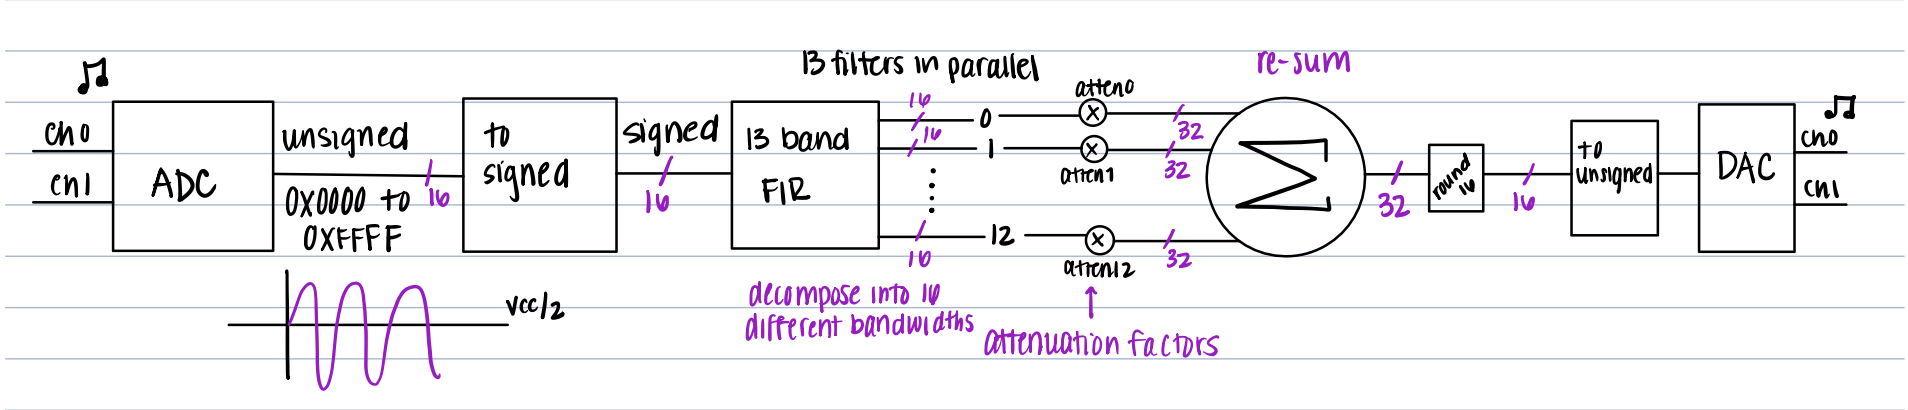
\includegraphics[width=0.9\linewidth]{Figures/EQ/signal_flow.png}
\caption{\label{fig:flow}Illustrated signal flow for the Audio Equalizer.}
\end{figure}

\subsection{Equalizer Components}\label{subsec:eq_comp}
\paragraph{Signal Converters} The equalizer utilizes an ADC to convert analog signals into digital, processable signals for the FIR filter. A DAC is used to convert the processed digital signals back to analog signals for audio output. The SPI modules that interface with the DAC and the ADC are properly configured using our previous work to sample at $100kHz$ overall, while $50kHz$ on each channel. Note that the Nyquist Sampling Criteria requires analog signals to be sampled at twice the source frequency. Since we are sampling human-audible signals that range from $2kHz$ to $20kHz$, a $50kHz$ sampling frequency meets this sampling criteria. 

Given our previous implementation of buffer memories in our SPI module, we significantly reduce the timing complexity of reading from or write to the signal converters. The equalizer module can read from or write to the signal converters anytime it sees fit, while the buffer memories keep the input/output data intact during the read/write operations.

\begin{figure*}[t]
    \centering
    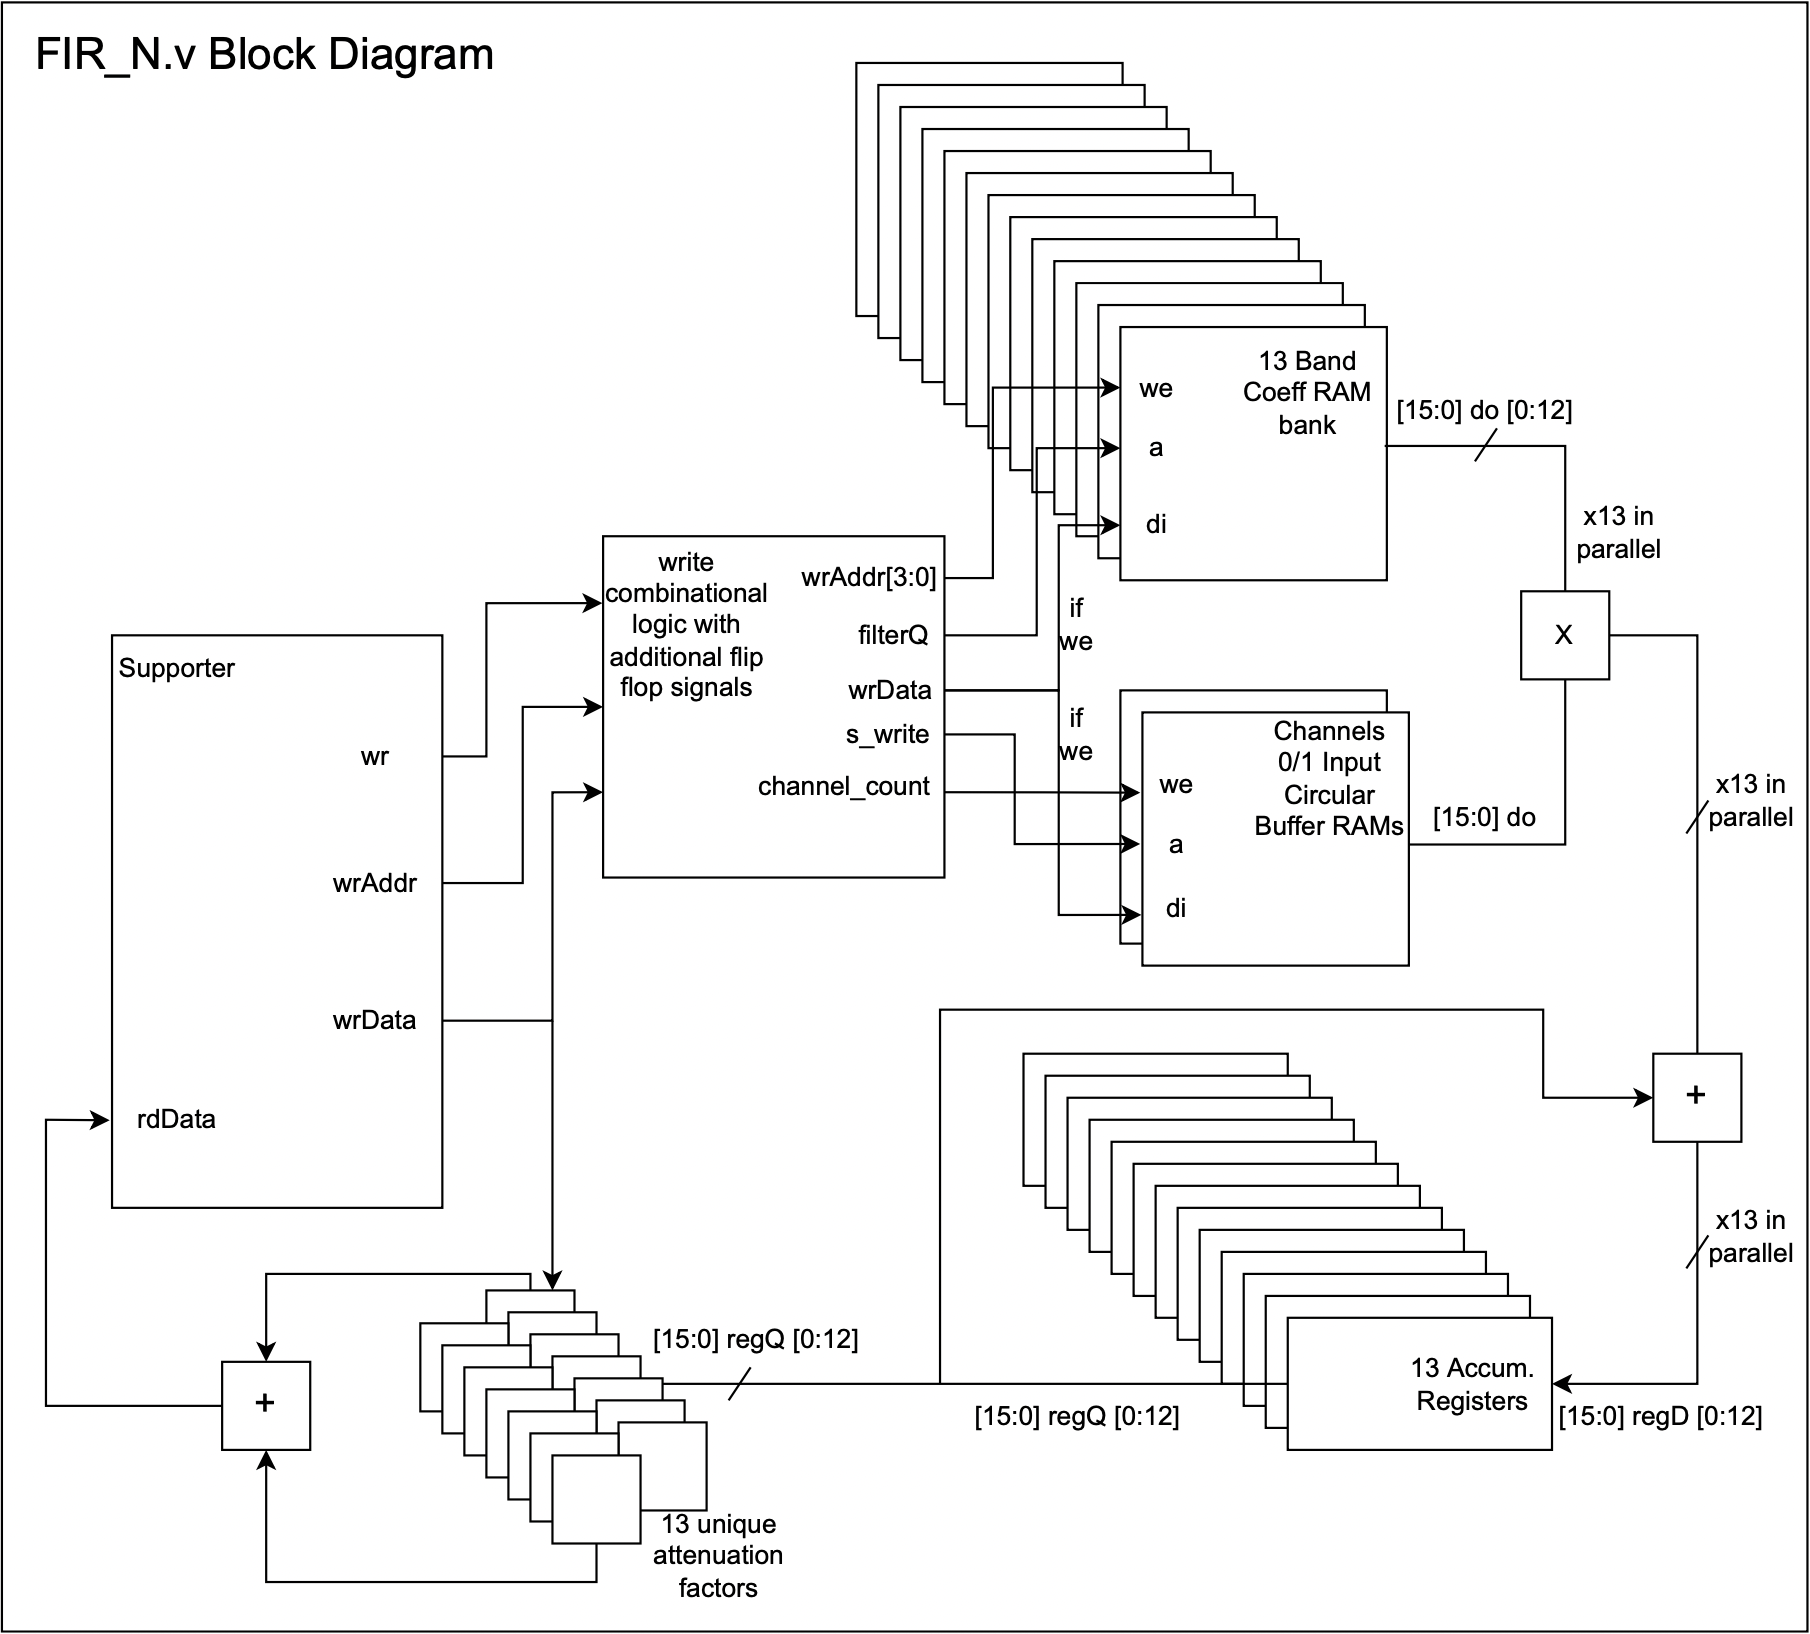
\includegraphics[width=0.7\linewidth]{Figures/EQ/fir_block.png}
    \caption{Block diagram for implemented FIR\_N module that uses 13 bands and 2 channels.}
    \label{fig:FIR_BLOCK}
\end{figure*}

\paragraph{Finite Impulse Response Filter}
Though our SPI module design remains unchanged, the FIR Filter design needs a significant expansion. An audio equalizer, by design, augments/attenuates specific frequency bands of a sound signal to achieve the desired audio effect. An equalizer can, for example, augment the ``base" of a song by boosting the magnitude of the lower frequency bands of the audio signal. 

To achieve band-specific attenuation/augmentation, we expand our previous, single-band FIR low-pass filter in two ways. First, we add in 12 additional band-pass filters that separate the audio signal into 13 frequency bands. The output signal, as a result, will be the sum of all outputs from all filters. Additional hardware such as extra storage units, rounding logic and summing logic are added as a result. Second, we add in additional write logic and storage to configure external attenuation constants. These attenuation constants target specific frequency bands and indicate if the magnitude within the band should whether be attenuated (with a less-than-one constant) or boosted (with a more-than-one constant). Since we wish to make our equalizer interactive, we equip the hardware with continuous read-write capabilities. The attenuation factors can be changed by a Microblaze\textregistered{} program at any given time. We again implement buffer memories to ease the timing constraint while ensure correct write timing. Fig~\ref{fig:FIR_BLOCK} shows the expanded architecture of the FIR filter, and Fig~\ref{fig:FIR_FSM} shows the updated logic design for the filter FSM.

\begin{figure*}[htbp]
\centering
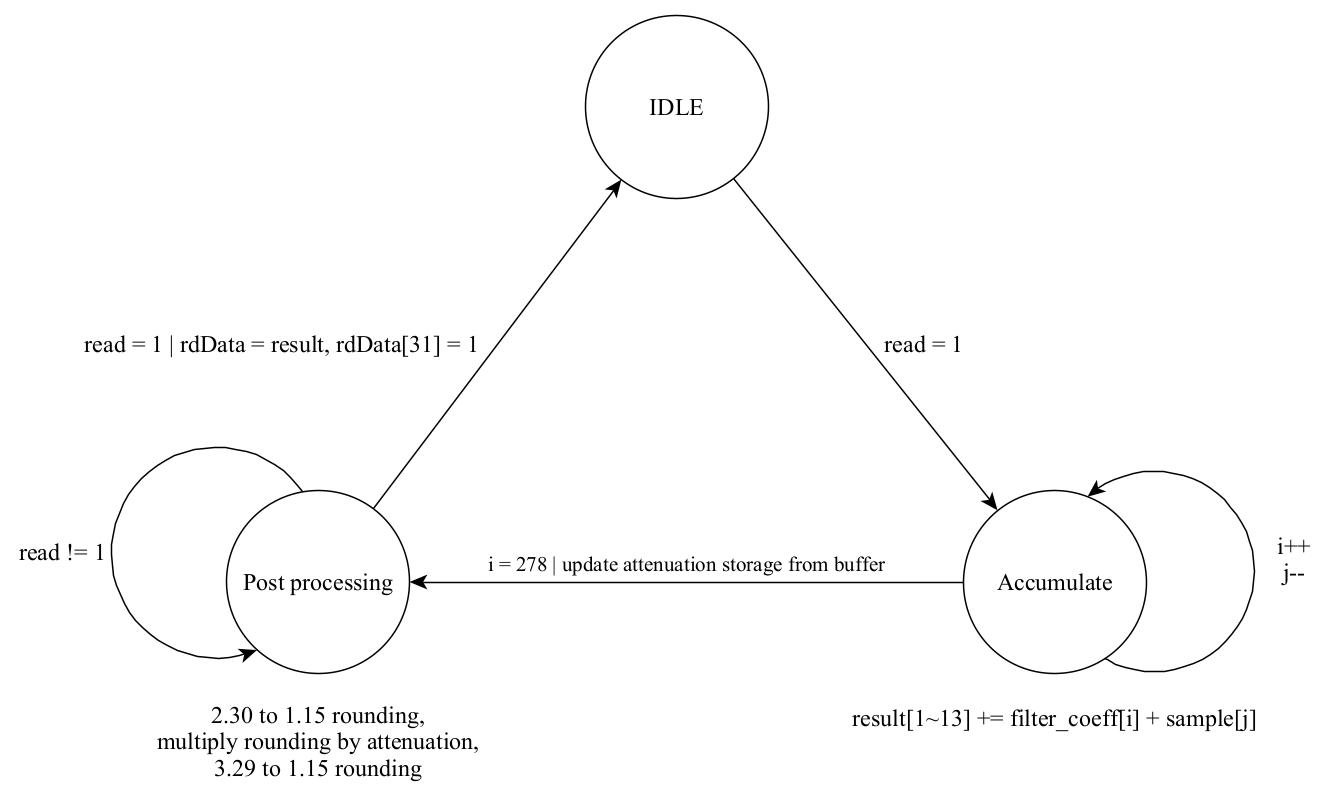
\includegraphics[width=0.9\linewidth]{Figures/EQ/fir_fsm.jpg}
\caption{\label{fig:FIR_FSM} Bubble Diagram for Filter FSM .}
\end{figure*}

\begin{figure*}[htbp]
\centering
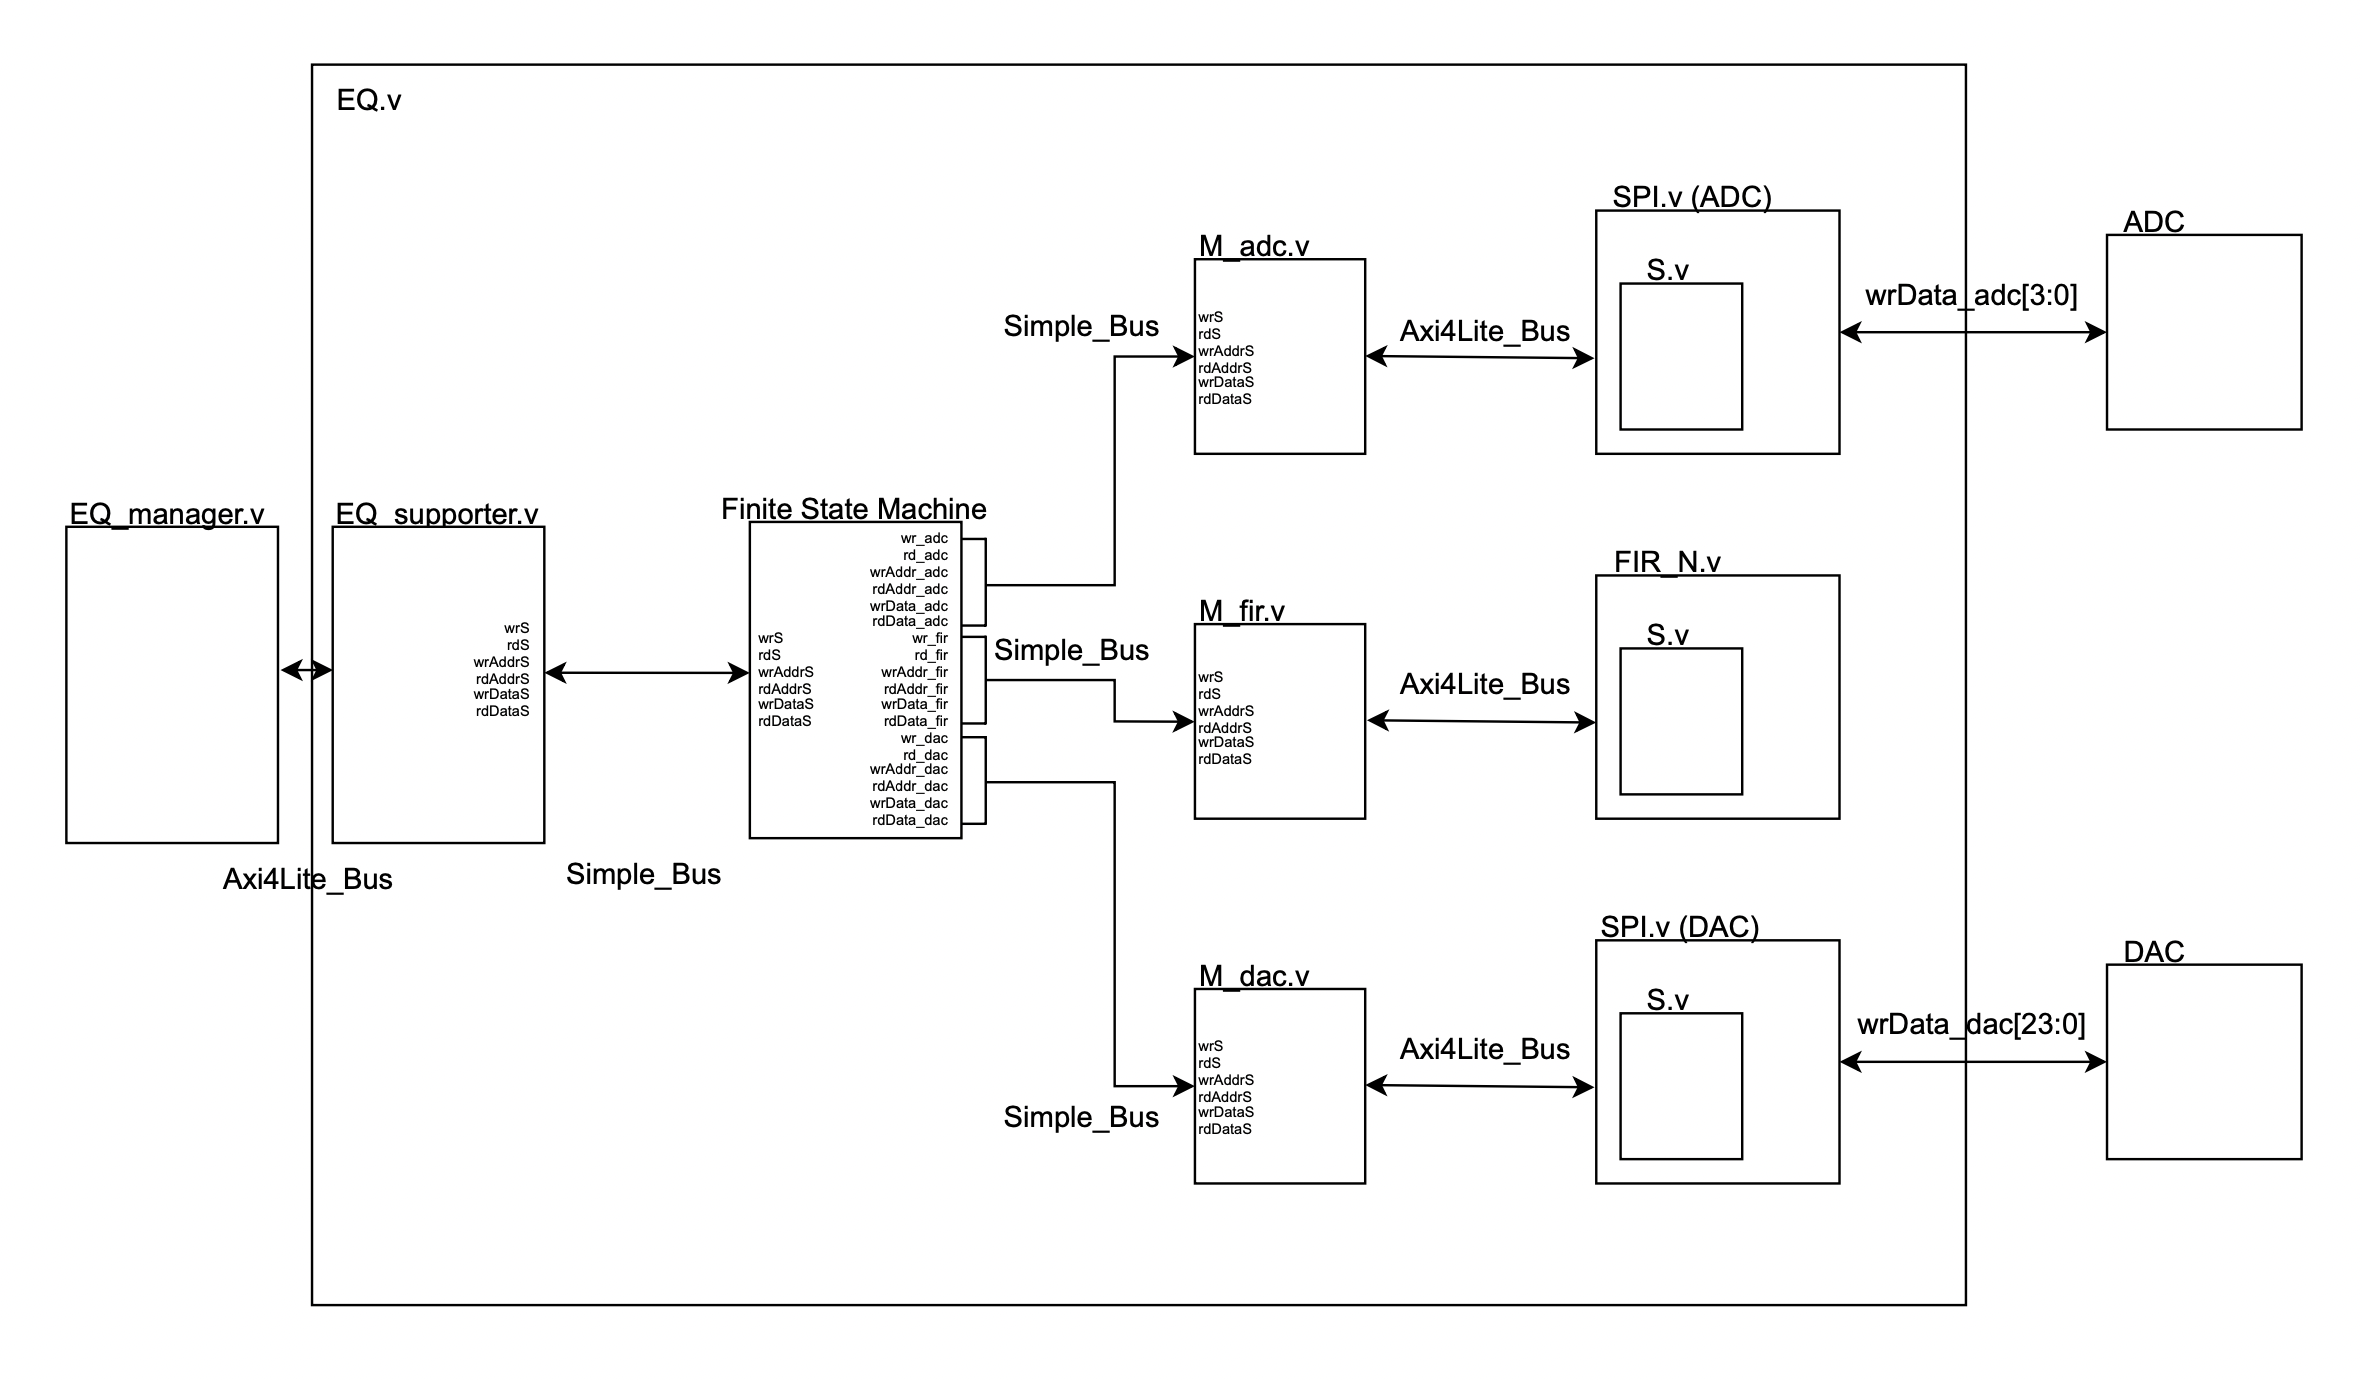
\includegraphics[width=0.9\linewidth]{Figures/EQ/eq_block.png}
\caption{\label{fig:EQ_BLOCK}Block diagram for entire module project with some abstraction conditional logic.}
\end{figure*}


\subsection{Device Design}\label{subsec:dev_design}
The 13-band audio equalizer combines two SPI modules and one FIR filter module. Fig.~\ref{fig:EQ_BLOCK} shows the hardware architecture of the equalizer module. Given that we have designed these modules in our previous assignments as Axi4Lite peripherals, we instantiated Axi4Lite managers to interface with each peripheral through Axi4Lite buses that are internal to our module. This design simplifies the equalizer control path design, as the equalizer only needs to send or receive simple bus signals to the instantiated Axi4Lite managers, which manage complex signals and and relevant timing requirements. Without managers, the equalizer will have to mimic a myriad of Axi4Lite bus signals under additional timing requirements. 

Serendipitously, instantiating filter module, SPI modules and their managers as separate entities enables the equalizer FSM to concurrently read or write from separate devices. Concurrent read or write between different modules reduces the signal transfer time required between each module, thus decreasing the timing complexity of the equalizer device logic.

\subsection{Device Timing}\label{subsec:dev_timing}
Given that the equalizer module interfaces with three different components, it is crucial for the equalizer module to conform to timing requirements. Table \ref{tbl:timing} shows the timing requirements posed by each components.


\begin{table}[htbp]
\caption{Overall Timing Constraints}
\scriptsize
\begin{center}
\begin{tabular}{|c|c|c|c|}
\hline
\multicolumn{4}{|c|}{\textbf{Minimum and Maximum Timing Requirements}}\\
\hline
Source & min/max & Value & Sequential/\\
& & & Concurrent \\
\hline
Signal sampling & min & $100kHz$ & \\
rate/period & & $300$ (clc cycle) & \\
\hline
Filter MAC & max & $279$ (clk cycle) & Sequential, \\
& & & must be after\\
& & & FIR write \\
\hline
Filter Read & max & $2$ (clk cycle) & Sequential,\\
& & & must happen after MAC\\
\hline
Filter Write & max & $1$ (clk cycle) & Sequential,\\
& & & must happen before MAC\\
\hline
DAC write & max & $1$ (clk cycle) & Sequential, \\
& & & must receive FIR \\
& & & result \\
\hline
ADC read & max & 3 (clk cycle) & Sequential, \\
& & & starts processing \\
\hline
& min & 2 (clk cycle) & Sequential \& concurrent, \\
ADC/DAC config & & each & must happen before ADC read,\\
& & & can be concurrent to \\
& & & DAC/FIR read/write \\
\hline
FIR config & max & 4185 (clk cycle) & Sequential \& concurrent, \\
& & & must happen before FIR ops,\\
& & & can be concurrent to \\
& & & ADC/DAC read/write\\
\hline
\end{tabular}
\label{tbl:timing}
\end{center}
\end{table}


Overall, four pieces of sequential operation post the most significant timing constraints. The overall, repeating operation sequence for sample processing can be described as: ADC Read \textrightarrow Filter Write \textrightarrow Filter MAC \textrightarrow Filter Read \textrightarrow DAC Write. These operations must happen in sequence, and must meet the $300$ clock cycle ($100kHz$ sampling rate) constraint between each ADC reads. We do meet this timing requirement, given that all four operations combined takes up $286$ clock cycles. We can further reduce the total time by concurrently reading from ADC and writing to Filter, as well as concurrently reading from Filter and writing to DAC. Though the SPI module provides DAC write confirmation, requiring such confirmation to move to the next sample processing cycle is not necessary, since sufficient time would have elapsed between two consecutive DAC writes. Based on these considerations, we design the following timing logic as described by the FSM in Fig.~\ref{fig:EQ_FSM}. The config stage, which contains all the necessary device configuration logic, concurrently configures the ADC, DAC and the filter to perform dual channel, 13-band, 279-term finite impulse response filtering at $100kHz$. After all configurations are done, the equalizer goes into the sampling loop, in which the equalizer sequentially receives, processes, and outputs audio signals. 

\begin{figure*}[htbp]
\centering
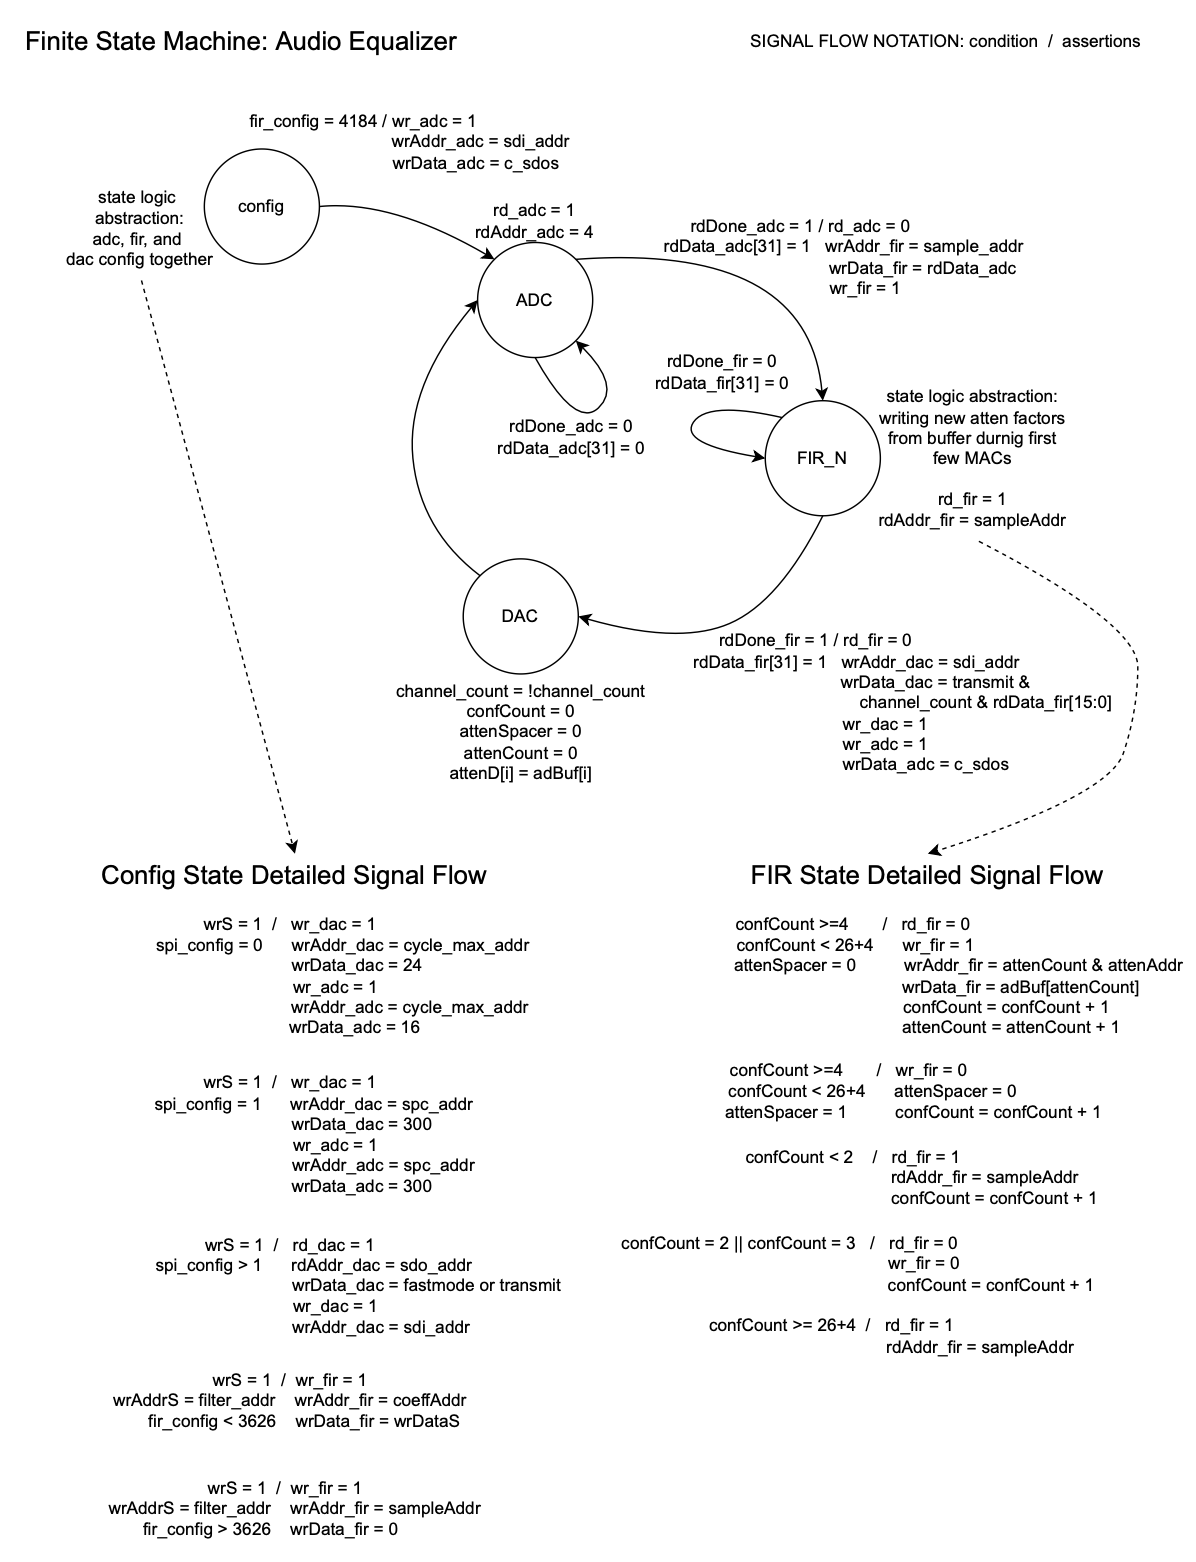
\includegraphics[width=0.9\linewidth]{Figures/EQ/eq_fsm.png}
\caption{\label{fig:EQ_FSM}Finite State Machine showing Equalizer states and state transition logic implemented.}
\end{figure*}

\section{Implementation and Operational Testing}\label{sec:implementation}
All C programs and simulation results were culminated in a hardware implementation of the Microblaze processor using a Field Programmable Gate Array (FPGA). Results from the hardware were amply tested for correct frequency response, filter results, functionality with a windows application graphical user interface (GUI), and functionality with the serial port communication between the FPGA and GUI.

\paragraph{Verilog Hardware Implementation}
To begin with the implementation process, we modify our previous FIR low-pass filter as outlined by section \ref{subsec:eq_comp}. The expanded filter module along with proper SPI module and their respective Axi4Lite managers are then properly connected internally to the equalizer. The FSM that governs the inputs and outputs of the equalizer unit is subsequently implemented, along with appropriate read/write logic that receives data from the Microblaze processor. 

Like our previous designs, the equalizer is implemented as an Axi4Lite peripheral connected to the Microblaze processor. The Verilog hardware description to each part can be found in the appendix.

\paragraph{Interface Code Implementation}
The interface to our equalizer peripheral serves two main functions: device configuration and attenuation factor configuration. The device interface is implemented in C. The interface first writes in the filter coefficients sequentially to the equalizer while concurrently writes in SPI configuration data (maximum sampling rate, control word length, etc). After proper configuration, the interface goes into a continuous receiver loop that listens for attenuation factor input through serial communication. When the interface receives a full packet (13 2-byte attenuation factors), the interface passes the factors to the equalizer peripheral, and goes back to the receiver loop.

\paragraph{Filter Testing} The first aspect of testing for the equalizer was to ensure that the modified FIR module to include 2 channels and 13 bands was properly producing the output sine wave. To do this, a C program was used to implemented the same filer in software to numerically compare with the hardware simulation results. The plotted output 1kHz sine waves from both the C program and the hardware simulation are shown in Fig.~\ref{fig:CvV}. The two sine waves are identical numerically, as shown by difference calculation and Fig.~\ref{fig:CvV}.

\begin{figure}[htbp]
\centering
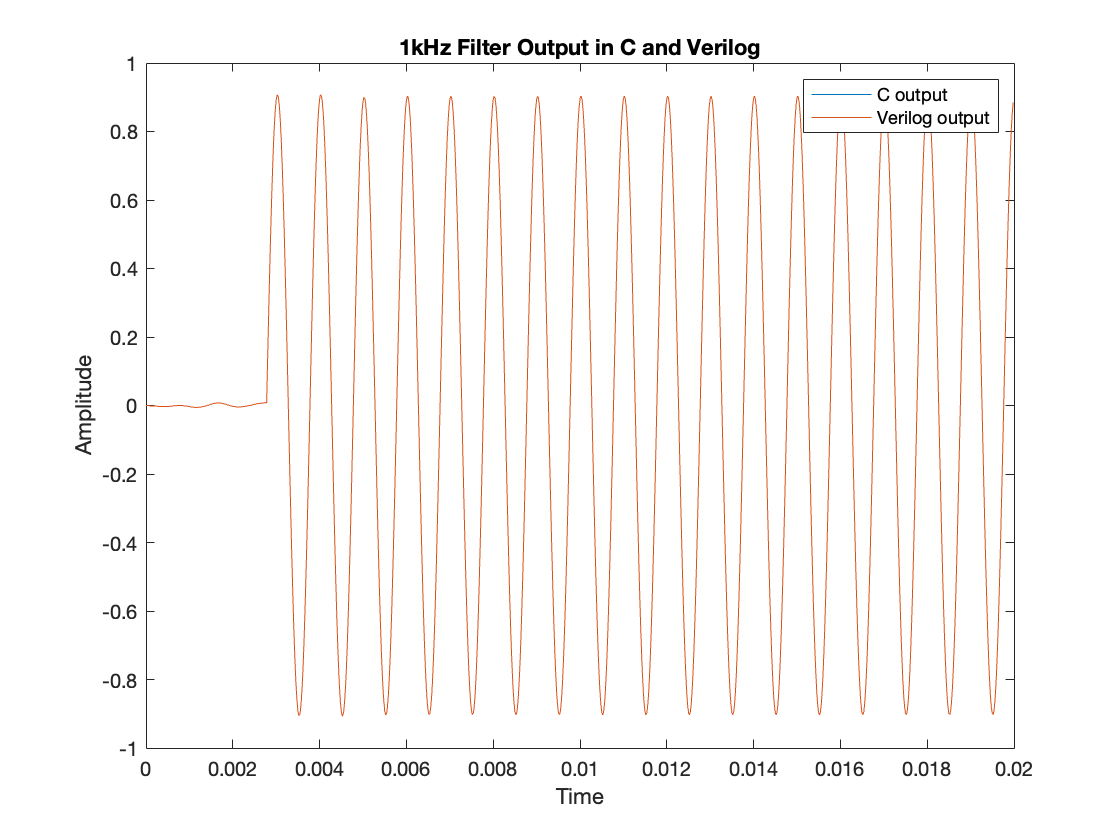
\includegraphics[width=0.9\linewidth]{Figures/EQ/CvsVerilog_output.png}
\caption{\label{fig:CvV}C implementation and hardware simulation output sine waves.}
\end{figure}

The second aspect testing was the expected phase lag from the input to the output. Because the FIR filter module has 279 taps for this 13 band filter, the expected phase lag can be calculated using \eqref{eq:lag}. From this, the expected phase lag is 0.00279 seconds. Experimental phase lag was calculated by plotting the input and output sine waves at 200Hz, as seen in Fig.\ref{fig:lag}. The first peak of each was compared, finding the exact data points at which they occur. The experimental phase lag was 0.00278 seconds. There is probably error in the preciseness of finding the point at the peak of each sine wave that would leave to a phase lag slightly off from the expected value. However, this value is close enough to the expected lag to accept for functionality testing.

\begin{equation}
    lag = \frac{279}{2*50,000\text{Hz}}
    \label{eq:lag}
\end{equation}{}

\begin{figure}[htbp]
\centering
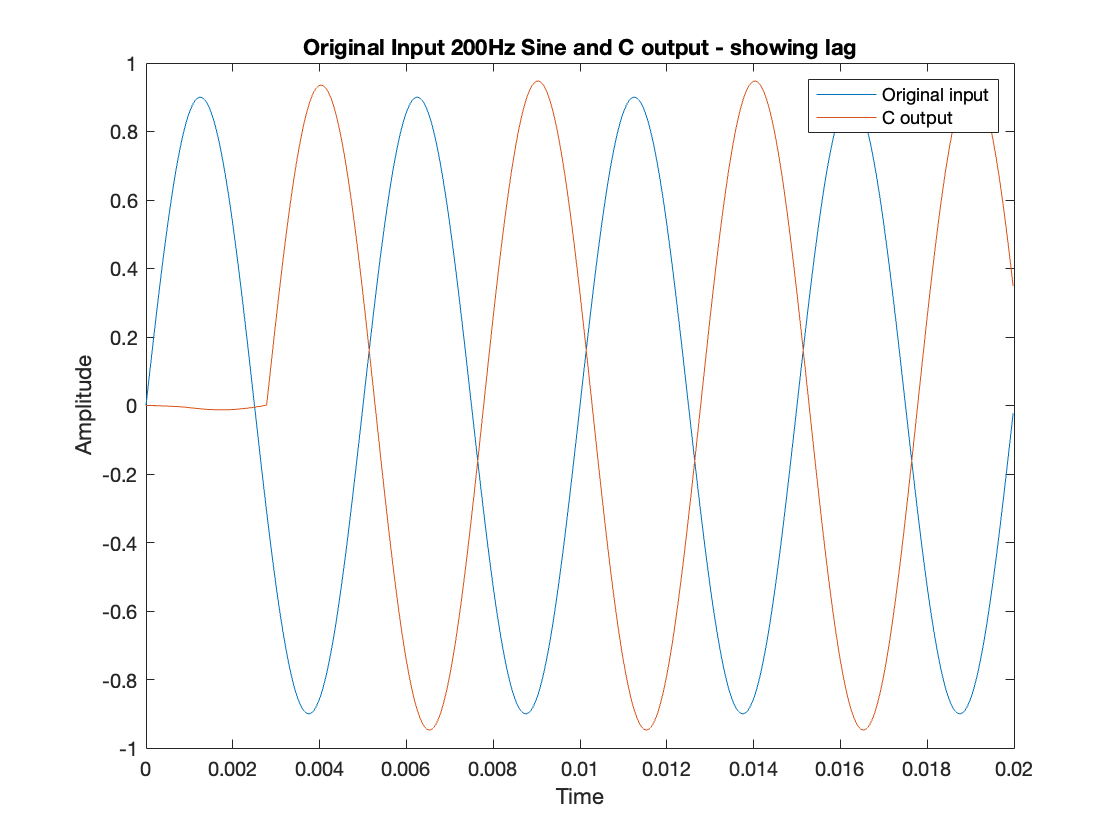
\includegraphics[width=0.9\linewidth]{Figures/EQ/outputLag.png}
\caption{\label{fig:lag}Input/output sine waves at 200Hz showing phase lag calculation.}
\end{figure}

\paragraph{Finite State Machine Testing}After ensuring the functionality of the modified FIR filter module, the audio equalizer finite state machine was tested as the equalizer was constructed. Because of the abundance of moving parts with this implementation, and therefore several complex states, it was necessary to test each state as it was created in the equalizer. Each state connected a new peripheral, firstly the ADC, secondly the FIR filter, and lastly the DAC. With each new state, the output of the peripheral was compared to previous output from that same module. For the ADC, results were tested with the ADC Tester module provided for the SPI project. After adding the FIR state, the simulation results were compared to previous testing results for just the FIR module modifications. For the DAC state, results were shown on the oscilloscope to ensure they matched as a time delayed version of the input from the function generator. This final state also served as one test for the whole equalizer since it also required the signal flowing through all implemented states to test the DAC. Additionally, for the DAC, the provided DAC Tester module from the SPI project was used to verify results. 

\paragraph{Frequency Response Testing} To ensure that the designed audio equalizer produced the correct frequency response from the Audio Equalizer Design Tool, two different comparison tests were performed. First, the natural output attenuation from the filter, without added attenuation factors, was compared against the expected attenuation. With all additional, band specific, attenuation factors set to 1, signifying no additional change, the output max value was compared to the input max value using \eqref{eq:db}. For this calculation, the filter produced 0.033599 dB of attenuation from the original signal, reasonably close to the expected value from the frequency response. 

\begin{equation}
    db = 20 \cdot \log_{10}(\frac{output}{input})
    \label{eq:db}
\end{equation}{}

Secondly, the function generator and oscilloscope were used to sweep the output frequencies. The FPGA was connected to the ADC and DAC peripherals with the function generator connected to the input of the ADC and the oscilloscope connected to the output of the DAC. Signals generated in the function generator were input to the audio equalizer through the ADC and displayed in comparison to a vertically shifted version of the original signal on the scope for verification. The mean amplitude value for the input and output sine waves were compared using \eqref{eq:db}. The table of expected dB attenuation based on the frequency response and collected dB attenuation during testing is shown below in \ref{tbl:attenuation}. An example image of the scope during this frequency response testing for 450Hz is shown in Fig.~\ref{fig:450_freq_resp}.

\begin{table}[htbp]
\caption{dB Attenuation in Frequency Response}
\begin{center}
\begin{tabular}{|c|c|c|}
\hline
\multicolumn{3}{|c|}{\textbf{Expected vs. Experimental Frequency Response}}\\
\hline
Frequency & Expected dB & Experimental dB\\
\hline
200Hz & 0.45 & 0.441\\
\hline
450Hz & -0.01 & -0.018\\
\hline
1300Hz & 0.25 & 0.254\\
\hline
\end{tabular}
\label{tbl:attenuation}
\end{center}
\end{table}

\begin{figure}[htbp]
\centering
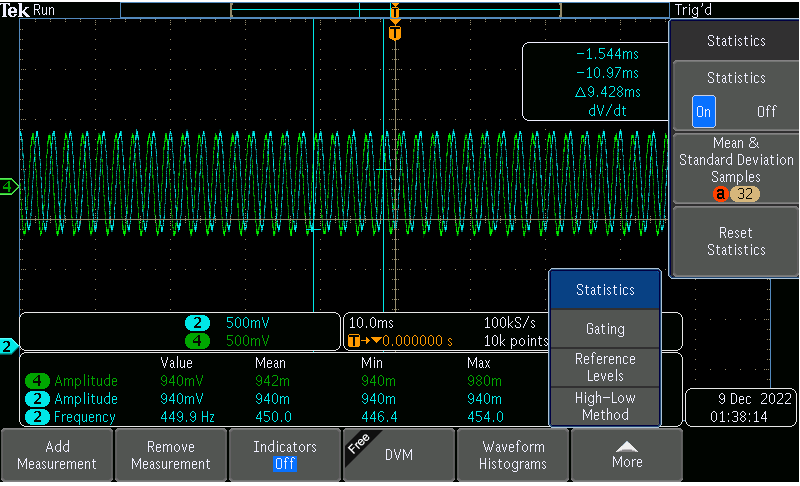
\includegraphics[width=0.9\linewidth]{Figures/EQ/450 Trough.PNG}
\caption{\label{fig:450_freq_resp}Input/output sine waves at 450Hz during frequency response testing.}
\end{figure}

The Filter design tool used for the initial filter coefficient creation was useful in comparing our results with the frequency response expected. An image of the magnitude and impulse responses of the designed 13 band filter is shown in Fig.~\ref{fig:magnitude}, and an image of the time domain and frequency domain responses to the filter are shown in Fig.~\ref{fig:domains}. Enlarging these images in the Filter Design Tool allowed comparison of the audio equalizer output to the correct frequency response for our Filter.

\begin{figure}[htbp]
\centering
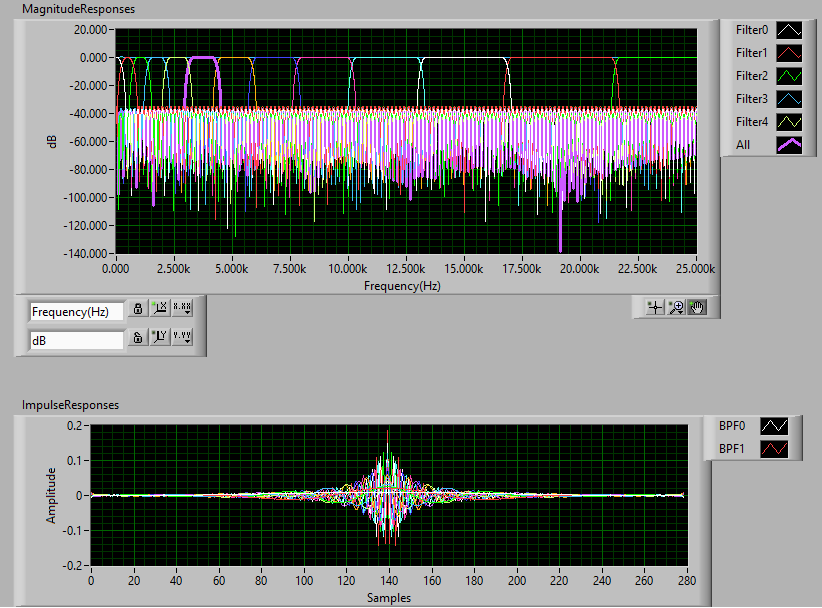
\includegraphics[width=0.9\linewidth]{Figures/EQ/magnitude.png}
\caption{\label{fig:magnitude}Magnitude and Impulse responses from the 13 band filter.}
\end{figure}

\begin{figure}[htbp]
\centering
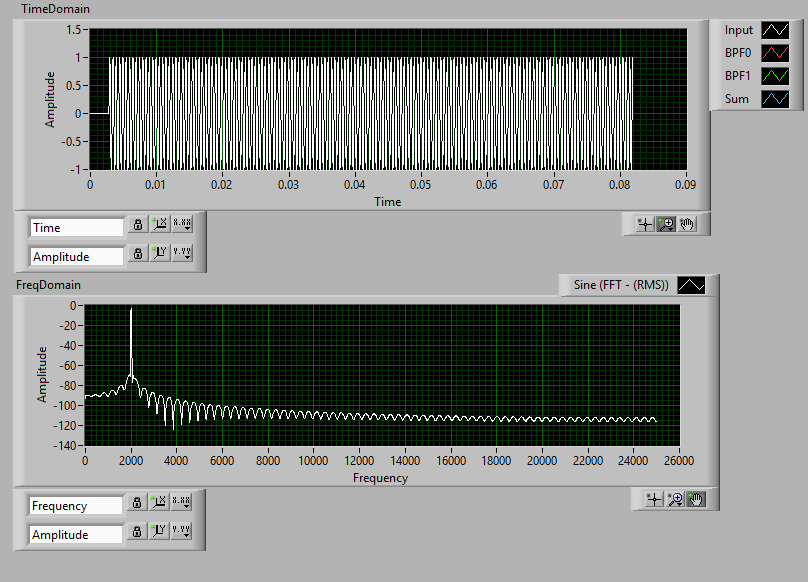
\includegraphics[width=0.9\linewidth]{Figures/EQ/freq_domain.png}
\caption{\label{fig:domains}Time and Frequency Domain responses from the 13 band filter.}
\end{figure}

\paragraph{Attenuation Testing} Once the finite state machine and frequency response were verified, the filter module was modified again to add dynamic attenuation factors. This allowed for serial port communication to change the attenuation factors used for the filter calculations, but also needed testing. The first test of the attenuation factors used just the modified filter module and the test bench used to test only that module while originally modifying it. The output of the filter was plotted again the input 1kHz sine wave to verify proper attenuation and valid data. Fig.~\ref{fig:half_sim} shows this verification plot for the 1kHz sine wave. 

To test the attenuation factors on the hardware with the whole equalizer, the function generator and oscilloscope were also used to display the input and output sine waves, as shown in Fig.~\ref{fig:half}. Both qualitatively and quantitatively, the output was analyzed against the input magnitude to ensure proper attenuation. In Fig.~\ref{fig:half}, it can be seen that the output, in blue, is half the amplitude of the input, in green. Various combinations of the set of 13 attenuation factors were used while the frequency was swept on the function generator. This allowed verification of attenuation at all of the 13 different frequency bands.

\begin{figure}[htbp]
\centering
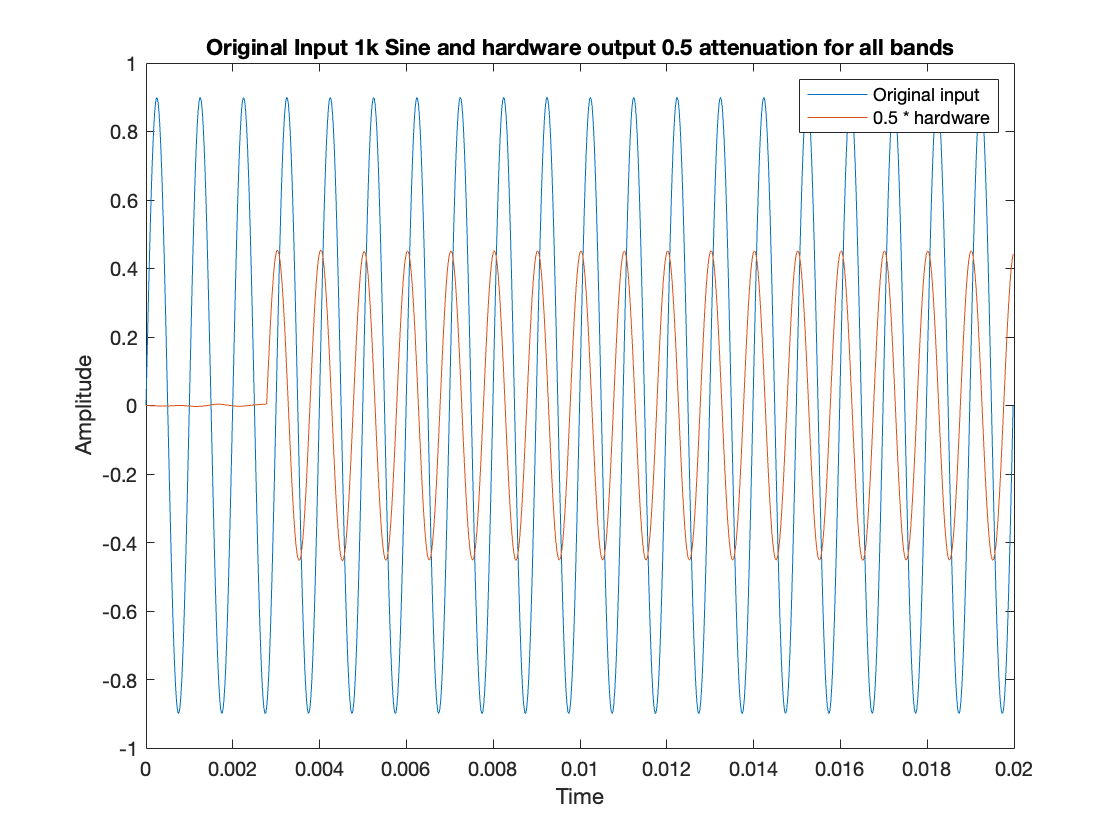
\includegraphics[width=0.9\linewidth]{Figures/EQ/output_atten.png}
\caption{\label{fig:half_sim}0.5 Attenuated output at 1.3kHz in filter simulation.}
\end{figure}

\begin{figure}[htbp]
\centering
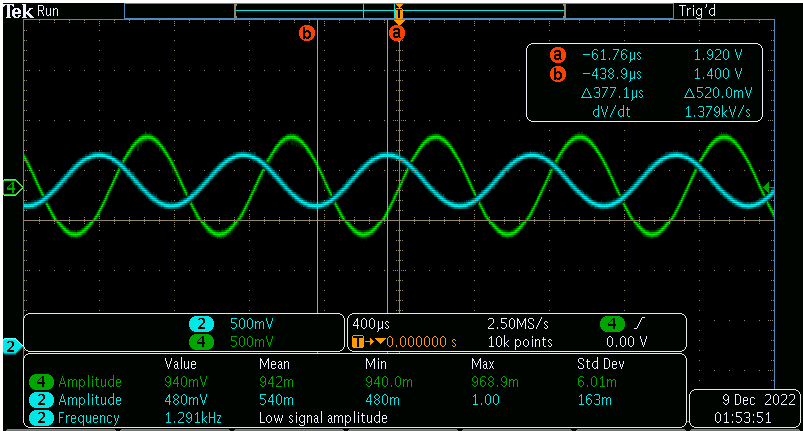
\includegraphics[width=0.9\linewidth]{Figures/EQ/half wave.PNG}
\caption{\label{fig:half}0.5 Attenuated output wave at 1.3kHz on Scope with hardware.}
\end{figure}

\paragraph{Windows Application} The final testing for the audio equalizer was to implement a GUI as a windows application to allow a user to interact with the equalizer while playing audio through the ADC. This primarily involved designing a front end and back end for the windows application to interact with the FPGA and peripherals through serial port communication. For our GUI, the application was designed using Python and its Tkinter framework. The backend of this application involved establishing a serial port communication connection to the Microblaze processor. The application then wrote the attenuation factors to be stored in the buffer for the filter to use in the filter state. Attenuation factors are written to the FPGA when the send button is clicked, sending the values of all 13 sliders.

UART serial communication only allowed us to send at most 16 bytes across the port in a single write operation. Because each attenuation factor is 2 bytes (4 hex nibbles), we were only able to send 8 attenuation factors at one time. To solve this, our application sends two consecutive writes and the module only finishes reading, allowing the attenuation factors to be used, once it has received 32 bytes.

The sliders in the application range from 0 to 100, where 0 represents attenuating the band entirely, therefore returning 0\% of the original signal, and 100 represents not attenuating the signal at all, therefore returning 100\% of the original signal. The GUI, with all sliders set at 100\% is shown in Fig.~\ref{fig:gui}. When the application is opened, or when the Reset Sliders button is pressed, all sliders default to 50, representing 50\% attenuation and therefore half the volume for all 13 frequency bands.

\begin{figure}[htbp]
\centering
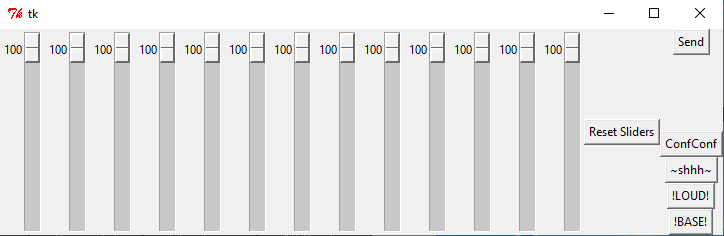
\includegraphics[width=0.9\linewidth]{Figures/EQ/gui.PNG}
\caption{\label{fig:gui}Windows Application with all attenuation factors at 100\% (no attenuation).}
\end{figure}

The buttons on the side add additional functionality such as presets for the sliders. The ``shhh" button sets all the sliders to 0, attenuating all the frequency bands to 0\% output when written to the equalizer by hitting the send button in the upper right corner in Fig.~\ref{fig:gui}. The ``!LOUD!" button sets all the sliders to 100. The ``!BASE!" button sets the sliders to a custom preset that amplifies the base frequencies in the input audio, as shown in Fig.~\ref{fig:preset}.

A special extra feature was implemented to add to the functionality of the windows application. The ``ConfConf" button accesses a secret mode that adds a new set of 13 sliders, one for each frequency band. Because the attenuation factors are designed to be from 0.0 to 1.0 inclusive, they must be implemented in 2.14 format. However, this also means that the attenuation factors can technically range from 0.0 to 1.99 inclusive. The ConfConf extra sliders allow a range from 0 to 190, instead of stopping at 100, and allowing the user to amplify the input signal at certain bands to 190\% of the original volume. This secret mode is shown in Fig.~\ref{fig:secret}. The EXTRA button, similar to the !LOUD! button in the normal mode, sets all sliders to 190\%. The EXTRA BASE button, similar to the !BASE! button in normal mode, sets sliders to the customized preset for base frequency amplification, as shown in Fig.~\ref{fig:secret}.

\begin{figure}[htbp]
\centering
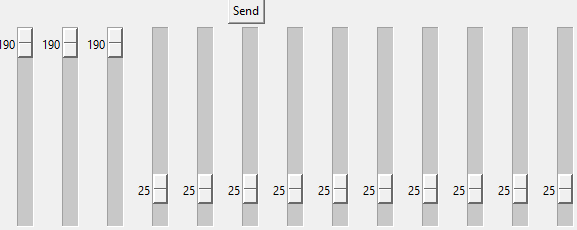
\includegraphics[width=0.9\linewidth]{Figures/EQ/presets.PNG}
\caption{\label{fig:preset}Base preset for sliders to amplify all base frequencies and attenuate others.}
\end{figure}

\begin{figure}[htbp]
\centering
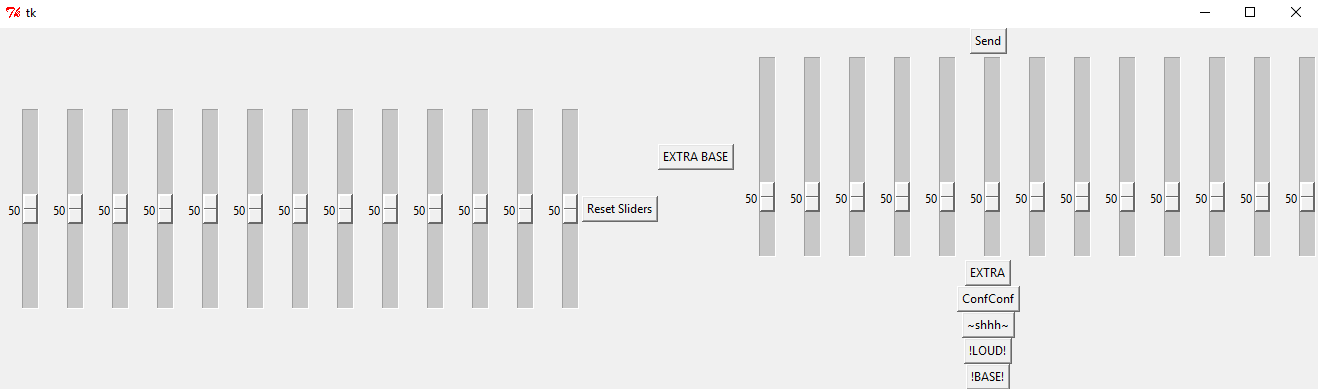
\includegraphics[width=0.9\linewidth]{Figures/EQ/secret mode.PNG}
\caption{\label{fig:secret}Additional Sliders in Secret Mode of Application for 190\% amplification capability.}
\end{figure}

Testing of the GUI included playing a song from a laptop through the FPGA and output from speakers. Audibly, it was verified that changing the sliders affected the sound of the output audio signal based on which attenuation factors were applied to which frequency bands. For example, changing all attenuation factors to 50\% caused the song output to play half as loud, changing all factors to be 0\% muted the song entirely, and using the custom base preset amplified the base in the song and attenuated the vocals.

\section{Discussion/Conclusion}\label{sec:discussion}
The Audio Equalizer combined various modules designed throughout the semester into a culminating hardware module and windows application GUI. This allows users to interact with the designed module to send specified audio through an ADC, FIR filter, and DAC to observe the resulting audio with 13 different frequency bands. Each band has the capability to be attenuated or amplified based on an attenuation factor between 0.0 and 1.0 inclusive, dynamically passed through the windows application sliders. The design and implementation of this module showed all of the timing requirements and design restrictions necessary when incorporating several different modules together to interact with one another. Each was modified, even if it was just slightly, to ensure compatibility for the overall audio equalizer. 

A single finite state machine controlled the data flow between all modules, ensure configuration in the first of four states, and then smooth, sequential transitions between states while processing the input audio signals. Every module was double buffered to allow for writing to the module at any point, and preventing timing conflicts and data corruption between states.

The overall project underwent ample testing at every step of design and implementation to ensure that the frequency response matched the designed 13 band filter, that all the components worked together without affecting the input signal, and that the audio played back with the appropriate attenuation factors. The final implementation is capable of playing a song through a speaker that dynamically attenuates chosen bands to amplify different frequencies in the song, such as base boasting to focus on the base frequencies of the song. The affect on each band can be visually seen by sweeping the frequencies in the function generator and watching the scope as each frequency is affected by its associated factor.

Future work for this project includes a real time feature for the windows application and pipelining for the equalizer finite state machine. Real time updating from the windows application would allow us to dynamically change the attenuation factors without having to hit the send button after adjusting the gains on the GUI sliders. The application would send the new values to the equalizer's attenuation factor buffer as an event listener when the sliders move. Additionally, pipelining the FSM for the whole equalizer would allow the module to be constantly working in all states, increasing the speed of processing. Currently, our FSM iterates through all three states after configuration, processing in each one individually before moving to the next. Pipelining would allow each state, and subsequently each peripheral, to be constantly processing either a current or upcoming signal.

\section*{Authors and Affiliations}\label{sec:authors}
The authors of this report, Will Wu and Cassie Jeng, can be reached at willwu@wustl.edu and jeng.c@wustl.edu, respectively.

\begin{thebibliography}{00}
    \bibitem{b1} 1st ed., vol. 2013, Xilinx, 2013, Vivado Design Suite User Guide.
    \bibitem{b2} Linear Technology, "Dual 14-Bit Rail-to-Rail DAC in 16-Lead SSOP Package," LTC1654. Linear Technology Corporation: Milpitas, CA.
    \bibitem{b3} Linear Technology, "$\mu$Power, 3V, 16-bit, 150ksps 1- and 2-Channel ADCs in MSOP," LTC1864L. Linear Technology Corporation: Milpitas, CA.
\end{thebibliography}

\textbf{For code, please see: \href{https://github.com/WillWu88/FPGA_Project_Reports/tree/main/Code/EQ}{Link to Github}}
\end{document}
